\documentclass[11pt]{article}
\usepackage{amsmath, amssymb, physics, mathtools, bm}
\usepackage{tikz}
\usetikzlibrary{decorations.pathmorphing,arrows.meta}
\usepackage[margin=2.3cm]{geometry}
\usepackage{siunitx, booktabs, hyperref}
\usepackage{braket}

\newcommand{\de}{\mathrm{d}}

\title{B3 Atomic and Laser Physics --- Model Solutions, Trinity Term 2022}
\author{}
\date{}

\begin{document}
\maketitle

\section*{Question 1 --- Sr terms, transitions, Zeeman}

\textbf{Problem.} (a) $LS$-coupling, dipole selection rules, terms of $5s^2,5s5p,5s6s$ in Sr. (b) Assign \SI{461}{nm}, \SI{679}{nm}, \SI{688}{nm}, \SI{707}{nm}, \SI{1.12}{\micro m}, \SI{689}{nm}; level diagram in $\si{m^{-1}}$; identify Normal Zeeman line. (c) $5s5d$ terms; allowed dipole transitions; identify the line splitting into 6 transverse-Zeeman components. (d) Practical apparatus.

\subsection*{(a)}

$LS$-coupling: residual electrostatic $\gg$ spin--orbit, so couple $\vb L=\sum\vb l_i$ and $\vb S=\sum\vb s_i$ first, then $\vb J=\vb L+\vb S$:
\[ H_\text{atom}\approx H_\text{c.f.}+H_\text{res}+H_\text{s.o.},\qquad H_\text{res}\gg H_\text{s.o.} \]
Good quantum numbers: $L,S,J,M_J$; term symbol ${}^{2S+1}L_J$. Valid for light atoms (small $Z$, since $H_\text{s.o.}\propto Z^4$).

General dipole rules (parity + rank-1 tensor):
\[ \Delta J=0,\pm1\;(0\nleftrightarrow 0),\quad \Delta M_J=0,\pm1,\quad \text{parity changes}. \]
$LS$-specific (dipole acts only on space):
\[ \Delta S=0,\quad \Delta L=0,\pm1\;(0\nleftrightarrow 0). \]

$5s^2$: equivalent closed sub-shell, Pauli forces $L=S=0$:
\[ {}^1S_0. \]
$5s5p$: inequivalent, $\ell_1=0,\ell_2=1$, $L=1$, $S=0,1$:
\[ {}^1P_1,\quad {}^3P_0,\;{}^3P_1,\;{}^3P_2. \]
$5s6s$: inequivalent, $\ell_1=\ell_2=0$, $L=0$, $S=0,1$:
\[ {}^1S_0,\quad {}^3S_1. \]

\subsection*{(b)}

Label $g={}^1S_0$ ($5s^2$), $a={}^1P_1$, $b={}^3P_0$, $c={}^3P_1$, $d={}^3P_2$, $e={}^3S_1$, $f={}^1S_0$ ($5s6s$).

\SI{461}{nm} seen in absorption from $g$: fully allowed singlet--singlet:
\[ g\to a:\;{}^1S_0\to{}^1P_1\;(\SI{461}{nm}). \]
\SI{689}{nm} weak from $g$: violates $\Delta S=0$ (intercombination):
\[ g\to c:\;{}^1S_0\to{}^3P_1\;(\SI{689}{nm}). \]
Remaining four lines connect $5s5p\leftrightarrow 5s6s$. Triplet--triplet allowed: ${}^3P_J\to{}^3S_1$ ($J=0,1,2$). Singlet--singlet allowed: ${}^1P_1\to{}^1S_0$. Land\'e interval rule on ${}^3P$ orders $J=0<1<2$:
\[ {}^3P_0\to{}^3S_1\;(\SI{679}{nm}),\;{}^3P_1\to{}^3S_1\;(\SI{688}{nm}),\;{}^3P_2\to{}^3S_1\;(\SI{707}{nm}),\;{}^1P_1\to{}^1S_0\;(\SI{1.12}{\micro m}). \]

Convert via $\tilde\nu=1/\lambda$ for $g\to a$:
\[ \tilde\nu_a=1/(461\times 10^{-9}\,\si{m})=\SI{2.169e6}{m^{-1}}. \]
For $g\to c$ (689 nm):
\[ \tilde\nu_c=1/(689\times 10^{-9}\,\si{m})=\SI{1.451e6}{m^{-1}}. \]
Convert 688 nm interval:
\[ 1/(688\times 10^{-9}\,\si{m})=\SI{1.453e6}{m^{-1}}. \]
Add 688 nm interval to $\tilde\nu_c$ to reach $e$:
\[ \tilde\nu_e=1.451\times 10^6+1.453\times 10^6=\SI{2.904e6}{m^{-1}}. \]
Convert 679 nm interval:
\[ 1/(679\times 10^{-9}\,\si{m})=\SI{1.473e6}{m^{-1}}. \]
Subtract from $\tilde\nu_e$ to reach $b$:
\[ \tilde\nu_b=2.904\times 10^6-1.473\times 10^6=\SI{1.431e6}{m^{-1}}. \]
Convert 707 nm interval:
\[ 1/(707\times 10^{-9}\,\si{m})=\SI{1.414e6}{m^{-1}}. \]
Subtract from $\tilde\nu_e$ to reach $d$:
\[ \tilde\nu_d=2.904\times 10^6-1.414\times 10^6=\SI{1.490e6}{m^{-1}}. \]
Convert 1.12 \si{\micro m} interval:
\[ 1/(1.12\times 10^{-6}\,\si{m})=\SI{0.893e6}{m^{-1}}. \]
Add to $\tilde\nu_a$ to reach $f$:
\[ \tilde\nu_f=2.169\times 10^6+0.893\times 10^6=\SI{3.062e6}{m^{-1}}. \]

\begin{center}
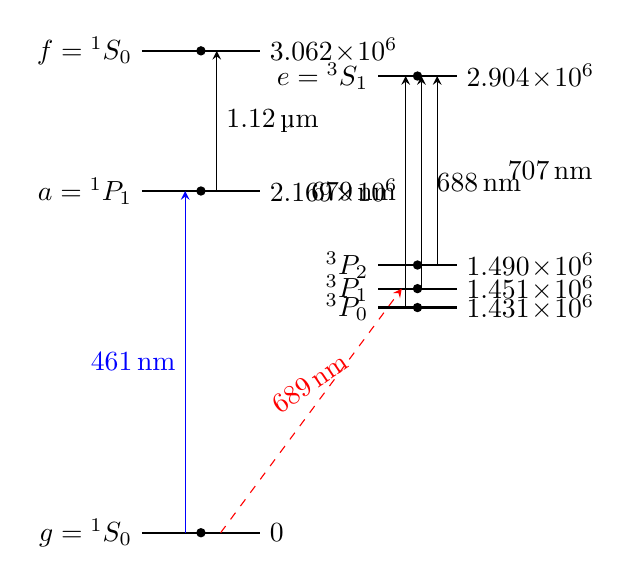
\begin{tikzpicture}[>=stealth, xscale=1.0, yscale=2.0]
% ground
\node[circle,fill,inner sep=1.2pt] (g) at (0.75,0) {};
\draw[thick] (0,0) -- (1.5,0);
\node[left] at (0,0) {$g={}^1S_0$};
\node[right] at (1.5,0) {$0$};
% triplet 5s5p
\node[circle,fill,inner sep=1.2pt] (b) at (3.5,1.43) {};
\draw[thick] (3,1.43) -- (4,1.43);
\node[left] at (3,1.43) {${}^3P_0$};
\node[right] at (4,1.43) {$1.431\!\times\!10^6$};
\node[circle,fill,inner sep=1.2pt] (c) at (3.5,1.55) {};
\draw[thick] (3,1.55) -- (4,1.55);
\node[left] at (3,1.55) {${}^3P_1$};
\node[right] at (4,1.55) {$1.451\!\times\!10^6$};
\node[circle,fill,inner sep=1.2pt] (d) at (3.5,1.70) {};
\draw[thick] (3,1.70) -- (4,1.70);
\node[left] at (3,1.70) {${}^3P_2$};
\node[right] at (4,1.70) {$1.490\!\times\!10^6$};
% singlet 5s5p
\node[circle,fill,inner sep=1.2pt] (a) at (0.75,2.17) {};
\draw[thick] (0,2.17) -- (1.5,2.17);
\node[left] at (0,2.17) {$a={}^1P_1$};
\node[right] at (1.5,2.17) {$2.169\!\times\!10^6$};
% 5s6s triplet
\node[circle,fill,inner sep=1.2pt] (e) at (3.5,2.90) {};
\draw[thick] (3,2.90) -- (4,2.90);
\node[left] at (3,2.90) {$e={}^3S_1$};
\node[right] at (4,2.90) {$2.904\!\times\!10^6$};
% 5s6s singlet
\node[circle,fill,inner sep=1.2pt] (f) at (0.75,3.06) {};
\draw[thick] (0,3.06) -- (1.5,3.06);
\node[left] at (0,3.06) {$f={}^1S_0$};
\node[right] at (1.5,3.06) {$3.062\!\times\!10^6$};
% transitions
\draw[->, blue] (0.55,0) -- (0.55,2.17) node[midway, left]{\SI{461}{nm}};
\draw[->, red, dashed] (1.0,0) -- (3.3,1.55) node[pos=0.55, above, sloped]{\SI{689}{nm}};
\draw[->] (3.35,1.43) -- (3.35,2.90) node[pos=0.5, left]{\SI{679}{nm}};
\draw[->] (3.55,1.55) -- (3.55,2.90) node[pos=0.5, right, xshift=2pt]{\SI{688}{nm}};
\draw[->] (3.75,1.70) -- (3.75,2.90) node[pos=0.5, right, xshift=22pt]{\SI{707}{nm}};
\draw[->] (0.95,2.17) -- (0.95,3.06) node[midway, right]{\SI{1.12}{\micro m}};
\end{tikzpicture}
\end{center}

Normal Zeeman: needs $g_J=1$ on both levels, i.e.\ $S=0$ on both. Only singlet--singlet line qualifies:
\[ \boxed{\;\SI{461}{nm}\;({}^1S_0\to{}^1P_1)\;\text{shows the Normal Zeeman effect.}\;} \]

\subsection*{(c)}

$5s5d$: inequivalent, $\ell_1=0,\ell_2=2$, $L=2$, $S=0,1$:
\[ {}^1D_2,\quad {}^3D_1,\;{}^3D_2,\;{}^3D_3. \]
Parity of $5s5d$ is even ($\sum\ell_i$ even); same as $5s^2,5s6s$. Parity rule forbids $5s5d\to 5s^2,\,5s6s$. Allowed only to $5s5p$ (odd). Apply $\Delta S=0$, $\Delta L=0,\pm1$, $\Delta J=0,\pm1$ ($0\nleftrightarrow 0$):
\begin{itemize}
\item ${}^1D_2\to{}^1P_1$.
\item ${}^3D_1\to{}^3P_0,{}^3P_1,{}^3P_2$.
\item ${}^3D_2\to{}^3P_1,{}^3P_2$.
\item ${}^3D_3\to{}^3P_2$.
\end{itemize}
Total: 7 dipole-allowed transitions.

Land\'e factors (use $g_J=1+[J(J+1)+S(S+1)-L(L+1)]/[2J(J+1)]$):
\[ g({}^3D_1)=1+\frac{2+2-6}{4}=\tfrac{1}{2}. \]
\[ g({}^3P_1)=1+\frac{2+2-2}{4}=\tfrac{3}{2}. \]
\[ g({}^3D_2)=1+\frac{6+2-6}{12}=\tfrac{7}{6}. \]
\[ g({}^3D_3)=1+\frac{12+2-6}{24}=\tfrac{4}{3}. \]
\[ g({}^3P_2)=1+\frac{6+2-2}{12}=\tfrac{3}{2}. \]
\[ g({}^1D_2)=g({}^1P_1)=1. \]

Transition shifts in field: $\hbar\omega=\hbar\omega_0+(g'M'-gM)\mu_B B$, with selection $\Delta M=0,\pm 1$ (and $0\to0$ forbidden when $\Delta J=0$). Transverse view shows all $\Delta M$ values; count distinct shifts.

Consider ${}^3D_1\to{}^3P_1$ ($J'=1\to J=1$, $g'=1/2$, $g=3/2$): pairs $(M',M)$ with $|M'-M|\le1$ excluding $0\to 0$. Enumerate shifts $g'M'-gM$:
\[ M'=1,M=1:\;1/2-3/2=-1. \]
\[ M'=1,M=0:\;1/2. \]
\[ M'=0,M=1:\;-3/2. \]
\[ M'=0,M=-1:\;3/2. \]
\[ M'=-1,M=0:\;-1/2. \]
\[ M'=-1,M=-1:\;-1/2+3/2=1. \]
Collect distinct shifts:
\[ \{\,-3/2,\,-1,\,-1/2,\,+1/2,\,+1,\,+3/2\,\}. \]
Exactly six distinct components:
\[ \boxed{\;{}^3D_1\to{}^3P_1:\text{ splits into 6 components in transverse view.}\;} \]
Reasoning: $0\to 0$ removal of the central $\pi$ line at $\Delta=0$ together with $g'\ne g$ giving paired $\pm$ shifts produces 6 distinct frequencies (no coincidences).

\subsection*{(d)}

Need resolution $\gtrsim \mu_B B/h\approx \SI{14}{GHz/T}$, i.e.\ $\sim\SI{1}{pm}$ at \SI{600}{nm}. Apparatus:
\begin{itemize}
\item Source: Sr hollow-cathode lamp or laser-excited atomic beam.
\item Magnet: water-cooled electromagnet, $B\sim$ \SIrange{0.1}{1}{T}, uniform over source.
\item Optics: collimation perpendicular to $\vb B$ (transverse view); polariser to separate $\pi$ ($\vb E\parallel\vb B$) and $\sigma$ ($\vb E\perp\vb B$).
\item Spectrometer: Fabry--P\'erot etalon (finesse $\gtrsim 30$), FSR matched to splitting; CCD detection.
\end{itemize}
Issues: Doppler broadening ($\sim\SI{1}{GHz}$ at \SI{600}{K}) must be smaller than the splitting---use cold atomic beam or laser cooling; calibrate $B$ (Hall probe / NMR); minimise pressure broadening.

\section*{Question 2 --- Hyperfine interval rule, Eu}

\textbf{Problem.} (a) $A\,\vb I\cdot\vb J$ interval rule; physical origins and good quantum numbers. (b) Why $4f^7 6s6d\,{}^8D_{11/2}$ has large hfs. (c) From peak table, show $a,b,c,e$ obey interval rule, find other ${}^{151}$Eu peaks, deduce $I({}^{151}\text{Eu})$. (d) $I({}^{153}\text{Eu})$ and $\mu_I$ ratio.

\subsection*{(a)}

Couple $\vb F=\vb I+\vb J$. Square:
\[ \vb F^2=\vb I^2+\vb J^2+2\,\vb I\cdot\vb J. \]
Solve for $\vb I\cdot\vb J$:
\[ \vb I\cdot\vb J=\tfrac{1}{2}\big(\vb F^2-\vb I^2-\vb J^2\big). \]
Eigenvalue in $\ket{IJFM_F}$:
\begin{equation}
E_F=\tfrac{1}{2}A\hbar^2\big[F(F+1)-I(I+1)-J(J+1)\big].
\label{eq:EF}
\end{equation}
Adjacent-level spacing from \eqref{eq:EF}:
\[ E_F-E_{F-1}=\tfrac{1}{2}A\hbar^2\big[F(F+1)-(F-1)F\big]. \]
Expand inside the bracket:
\[ F(F+1)-(F-1)F=F^2+F-F^2+F=2F. \]
Substitute back:
\begin{equation}
E_F-E_{F-1}=A\hbar^2 F.
\label{eq:interval}
\end{equation}
\boxed{\;\text{Spacing }\propto F:\text{ interval rule.}\;}

\paragraph{Origins.}
\begin{itemize}
\item Spin--orbit $\zeta(r)\,\vb L\cdot\vb S$: fine structure within an $LS$ term; good quantum numbers $L,S,J,M_J$; energy $\sim\SI{e-3}{eV}$ to $\sim\SI{1}{eV}$.
\item Magnetic-dipole hyperfine $A\,\vb I\cdot\vb J$: hyperfine multiplet within a level; good quantum numbers $I,J,F,M_F$; energy $\sim\si{\micro eV}$--$\si{meV}$ (RF/microwave).
\end{itemize}

\subsection*{(b)}

Two factors:
\begin{itemize}
\item $4f^7$ half-filled shell: 7 unpaired spins giving large spin hyperfine field at the nucleus.
\item Unpaired $6s$ electron: $|\psi_{6s}(0)|^2\ne 0$ produces a large Fermi-contact interaction:
\[ A_{6s}\propto |\psi_{6s}(0)|^2\,\mu_I. \]
\end{itemize}
Combined effect makes $A$ unusually large.

\subsection*{(c)}

Lower level has negligible hfs, so transition frequencies map to upper-level $E_F$ via \eqref{eq:EF}. Compute pairwise differences along $a,b,c,e$:
\[ \nu_a-\nu_b=21.19-18.37=\SI{2.82}{GHz}. \]
\[ \nu_b-\nu_c=18.37-14.84=\SI{3.53}{GHz}. \]
\[ \nu_c-\nu_e=14.84-10.60=\SI{4.24}{GHz}. \]
Form ratios with smallest:
\[ 2.82:3.53:4.24=4:5:6. \]
Matches \eqref{eq:interval} with $A'\equiv A\hbar^2/h$ (smallest spacing labelled by lower $F$ of the pair):
\[ A'=2.82/4=\SI{0.705}{GHz}. \]
Three consecutive spacings of magnitudes $4A',5A',6A'$ correspond to four adjacent $F$ levels (the $F$ in $E_F-E_{F-1}=A'F$ takes values $4,5,6$). The four peaks $a,b,c,e$ therefore correspond to $F\in\{3,4,5,6\}$ in the upper level (ordered with the larger spacings at lower frequency since $A<0$ here, giving $F_a=3,F_b=4,F_c=5,F_e=6$).

Predict next interval ($F=7$ gives spacing $7A'$):
\[ \Delta_{67}=7\times 0.705=\SI{4.94}{GHz}. \]
Position of $F=7$ peak:
\[ \nu_e-\Delta_{67}=10.60-4.94=\SI{5.66}{GHz}\;\rightarrow\;i\;(5.63). \]
Predict next ($F=8$, spacing $8A'$):
\[ \Delta_{78}=8\times 0.705=\SI{5.64}{GHz}. \]
Position of $F=8$ peak:
\[ \nu_i-\Delta_{78}=5.63-5.64\approx 0.0\;\rightarrow\;l. \]
${}^{151}$Eu peaks therefore:
\[ \boxed{\;\{a,b,c,e,i,l\}.\;} \]
Six adjacent $F$ values ($F=3$ to $F=8$) require:
\[ 2I+1=6. \]
Solve for $I$:
\[ \boxed{\;I({}^{151}\text{Eu})=\tfrac{5}{2}.\;} \]
Check: $F_\text{max}=J+I=11/2+5/2=8$, $F_\text{min}=|J-I|=11/2-5/2=3$, consistent.

\subsection*{(d)}

Remaining peaks $\{d,f,g,h,j,k\}$ at $10.99,9.74,8.17,6.29,4.09,1.58\,\si{GHz}$. Compute consecutive differences:
\[ \nu_d-\nu_f=10.99-9.74=\SI{1.25}{GHz}. \]
\[ \nu_f-\nu_g=9.74-8.17=\SI{1.57}{GHz}. \]
\[ \nu_g-\nu_h=8.17-6.29=\SI{1.88}{GHz}. \]
\[ \nu_h-\nu_j=6.29-4.09=\SI{2.20}{GHz}. \]
\[ \nu_j-\nu_k=4.09-1.58=\SI{2.51}{GHz}. \]
Form ratios:
\[ 1.25:1.57:1.88:2.20:2.51=4:5:6:7:8. \]
Five spacings labelled $4,5,6,7,8$ imply six adjacent $F$ levels ($F=3$ to $F=8$):
\[ 2I+1=6. \]
Solve for $I$:
\[ \boxed{\;I({}^{153}\text{Eu})=\tfrac{5}{2}.\;} \]
Identify $A'_{153}$ from the smallest spacing ($F=4$):
\[ A'_{153}=1.25/4=\SI{0.3125}{GHz}. \]
Same $J$ and same $I$ for both isotopes, so $A\propto \mu_I/I$ with identical $I$:
\[ \frac{A_{151}}{A_{153}}=\frac{\mu_I({}^{151}\text{Eu})}{\mu_I({}^{153}\text{Eu})}. \]
Substitute the two $A'$ values:
\[ \frac{\mu_I({}^{151}\text{Eu})}{\mu_I({}^{153}\text{Eu})}=\frac{0.705}{0.3125}. \]
Evaluate:
\[ \boxed{\;\frac{\mu_I({}^{151}\text{Eu})}{\mu_I({}^{153}\text{Eu})}\approx 2.26.\;} \]

\section*{Question 3 --- Two-level atom in classical field}

\textbf{Problem.} Two-state atom driven by $\hat D_0\cos\omega t$; $\Psi=c_1\psi_1 e^{-iE_1 t/\hbar}+c_2\psi_2 e^{-iE_2 t/\hbar}$. (a) Sudden switch-on with $c_1(0)=1$: find $|c_2|^2=U\sin^2(\alpha t)$ under $|\omega-\omega_0|\ll\omega_0$, give $U,\alpha$, and $\tau\to\infty$ time average. (b) Rabi vs.\ Einstein. (c) Lorentzian from natural broadening (Fourier); another mechanism. (d) Pulse $\hat D_0 e^{-b|t|}\cos\omega t$, weak field: $c_2(t>0)$, $|c_2(\infty)|^2$, FWHM.

\subsection*{(a)}

Project TDSE onto $\psi_{1,2}$ using $\bra{\psi_i}\hat D_0\ket{\psi_i}=0$:
\[ i\hbar\dot c_2=D_{21}\cos(\omega t)\,e^{i\omega_0 t}\,c_1. \]
\[ i\hbar\dot c_1=D_{12}\cos(\omega t)\,e^{-i\omega_0 t}\,c_2. \]
Expand the cosine:
\[ \cos\omega t=\tfrac{1}{2}\big(e^{i\omega t}+e^{-i\omega t}\big). \]
Apply RWA (drop $e^{\pm i(\omega+\omega_0)t}$, valid for $|\omega-\omega_0|\ll\omega_0$):
\begin{equation}
i\hbar\dot c_2=\tfrac{1}{2}D_{21}\,e^{-i\delta t}c_1,\qquad i\hbar\dot c_1=\tfrac{1}{2}D_{12}\,e^{i\delta t}c_2,\qquad \delta=\omega-\omega_0.
\label{eq:RWA}
\end{equation}
Define on-resonance Rabi frequency:
\[ \Omega_0\equiv|D_{21}|/\hbar. \]
Differentiate the $c_2$ equation in time:
\[ i\hbar\ddot c_2=\tfrac{1}{2}D_{21}\big(-i\delta\big)e^{-i\delta t}c_1+\tfrac{1}{2}D_{21}e^{-i\delta t}\dot c_1. \]
Substitute $\dot c_1$ from \eqref{eq:RWA}:
\[ i\hbar\ddot c_2=-i\delta\,i\hbar\dot c_2+\tfrac{1}{2}D_{21}e^{-i\delta t}\cdot\frac{D_{12}e^{i\delta t}c_2}{2i\hbar}. \]
Simplify the second term using $|D_{21}|^2=\hbar^2\Omega_0^2$:
\[ i\hbar\ddot c_2=-i\delta\,i\hbar\dot c_2-\frac{i\hbar\Omega_0^2}{4}c_2. \]
Divide through by $i\hbar$:
\[ \ddot c_2+i\delta\,\dot c_2+\tfrac{1}{4}\Omega_0^2 c_2=0. \]
Initial conditions: $c_2(0)=0$ and $\dot c_2(0)=-i\Omega_0/2$ from \eqref{eq:RWA} with $c_1(0)=1$. Try $c_2(t)=e^{-i\delta t/2}f(t)$:
\[ \ddot f+\tfrac{1}{4}(\Omega_0^2+\delta^2)f=0. \]
Define generalised Rabi frequency:
\[ \Omega\equiv\sqrt{\Omega_0^2+\delta^2}. \]
General solution $f=A\cos(\Omega t/2)+B\sin(\Omega t/2)$; impose $f(0)=0$:
\[ A=0. \]
Impose $\dot f(0)=\dot c_2(0)=-i\Omega_0/2$ (since $f(0)=0$):
\[ B\Omega/2=-i\Omega_0/2\;\Longrightarrow\;B=-i\Omega_0/\Omega. \]
Combine:
\begin{equation}
c_2(t)=-\frac{i\Omega_0}{\Omega}\,e^{-i\delta t/2}\sin(\tfrac{1}{2}\Omega t).
\label{eq:c2}
\end{equation}
Take modulus squared:
\[ |c_2(t)|^2=\frac{\Omega_0^2}{\Omega_0^2+\delta^2}\sin^2(\tfrac{1}{2}\Omega t). \]
Read off $U$ and $\alpha$:
\[ \boxed{\;U=\frac{\Omega_0^2}{\Omega_0^2+\delta^2},\qquad \alpha=\tfrac{1}{2}\sqrt{\Omega_0^2+(\omega-\omega_0)^2}.\;} \]

Use $\sin^2(\alpha t)=\tfrac{1}{2}(1-\cos 2\alpha t)$:
\[ \overline{|c_2|^2}=\frac{U}{\tau}\int_0^\tau\sin^2(\alpha t)\,\de t. \]
Evaluate the integral:
\[ \overline{|c_2|^2}=\frac{U}{2}\left[1-\frac{\sin(2\alpha\tau)}{2\alpha\tau}\right]. \]
Take $\tau\to\infty$ (oscillatory term vanishes):
\[ \boxed{\;\lim_{\tau\to\infty}\overline{|c_2|^2}=\frac{U}{2}=\frac{\Omega_0^2}{2(\Omega_0^2+\delta^2)}.\;} \]

\subsection*{(b)}

Rabi oscillations require:
\begin{itemize}
\item Coherent monochromatic field ($\omega$ well defined).
\item Rabi period $\ll$ decoherence time: $\Omega T_2\gg 1$.
\item Interaction time $\gtrsim 1/\Omega$.
\end{itemize}
Einstein rate equations apply when:
\begin{itemize}
\item Broad-spectrum incoherent radiation, $u(\omega)$ slowly varying over linewidth.
\item Decoherence dominates: $\Omega\ll 1/T_2$, i.e.\ phase memory destroyed between events.
\item Recovered by adiabatic elimination of coherences in the density-matrix description.
\end{itemize}

\subsection*{(c)}

Decaying upper-state amplitude:
\[ \psi(t)=\psi_0\,e^{-i\omega_0 t}\,e^{-\Gamma t/2}\,\Theta(t),\qquad \Gamma=1/\tau. \]
Fourier transform:
\[ \tilde\psi(\omega)=\int_0^\infty \psi_0\,e^{i\omega t}e^{-i\omega_0 t}e^{-\Gamma t/2}\,\de t. \]
Combine exponents:
\[ \tilde\psi(\omega)=\psi_0\int_0^\infty e^{[i(\omega-\omega_0)-\Gamma/2]t}\,\de t. \]
Evaluate the integral:
\[ \tilde\psi(\omega)=\frac{\psi_0}{\Gamma/2-i(\omega-\omega_0)}. \]
Take modulus squared:
\[ |\tilde\psi(\omega)|^2=\frac{|\psi_0|^2}{(\Gamma/2)^2+(\omega-\omega_0)^2}. \]
Read off Lorentzian profile:
\[ \boxed{\;I(\omega)\propto\frac{1}{(\omega-\omega_0)^2+(\Gamma/2)^2}\;\text{(Lorentzian, FWHM }=\Gamma).\;} \]

Another Lorentzian mechanism: \textbf{collisional (pressure) broadening}. Random phase-interrupting collisions truncate the radiating dipole at exponential intervals; the autocorrelation decays as $e^{-\Gamma_\text{coll}t}$, giving a Lorentzian of width $\Gamma_\text{coll}=2/\tau_\text{coll}$.

\subsection*{(d)}

First-order perturbation with $c_1\approx 1$ and $c_2(-\infty)=0$:
\[ c_2(t)=\frac{1}{i\hbar}\int_{-\infty}^t D_{21}\,e^{-b|t'|}\cos(\omega t')\,e^{i\omega_0 t'}\,\de t'. \]
Apply RWA (keep $e^{-i\omega t'}$ piece of the cosine):
\[ c_2(t)=\frac{D_{21}}{2i\hbar}\int_{-\infty}^t e^{-b|t'|}e^{i(\omega_0-\omega) t'}\,\de t'. \]
Define detuning $\delta=\omega-\omega_0$:
\[ c_2(t)=\frac{D_{21}}{2i\hbar}\int_{-\infty}^t e^{-b|t'|}e^{-i\delta t'}\,\de t'. \]
Split the integral at $t'=0$ for $t>0$:
\[ c_2(t)=\frac{D_{21}}{2i\hbar}\left[\int_{-\infty}^0 e^{(b-i\delta)t'}\,\de t'+\int_0^t e^{-(b+i\delta)t'}\,\de t'\right]. \]
Evaluate each integral:
\begin{equation}
c_2(t)=\frac{D_{21}}{2i\hbar}\left[\frac{1}{b-i\delta}+\frac{1-e^{-(b+i\delta)t}}{b+i\delta}\right].
\label{eq:c2-finite}
\end{equation}
Take $t\to\infty$ (second exponential vanishes since $b>0$):
\[ c_2(\infty)=\frac{D_{21}}{2i\hbar}\left[\frac{1}{b-i\delta}+\frac{1}{b+i\delta}\right]. \]
Add the fractions:
\[ c_2(\infty)=\frac{D_{21}}{2i\hbar}\cdot\frac{(b+i\delta)+(b-i\delta)}{b^2+\delta^2}. \]
Simplify the numerator:
\[ c_2(\infty)=\frac{D_{21}}{2i\hbar}\cdot\frac{2b}{b^2+\delta^2}=\frac{D_{21}}{i\hbar}\cdot\frac{b}{b^2+\delta^2}. \]
Take modulus squared:
\[ \boxed{\;|c_2(\infty)|^2=\frac{|D_{21}|^2}{\hbar^2}\cdot\frac{b^2}{(b^2+\delta^2)^2}.\;} \]
This is a squared Lorentzian in $\delta$.

Maximum at $\delta=0$:
\[ |c_2(\infty)|^2_{\max}=\frac{|D_{21}|^2}{\hbar^2 b^2}. \]
Half-max condition $|c_2|^2=\tfrac{1}{2}|c_2|^2_{\max}$:
\[ \frac{b^2}{(b^2+\delta_{1/2}^2)^2}=\frac{1}{2 b^2}. \]
Rearrange:
\[ (b^2+\delta_{1/2}^2)^2=2 b^4. \]
Take positive square root:
\[ b^2+\delta_{1/2}^2=b^2\sqrt 2. \]
Solve for $\delta_{1/2}^2$:
\[ \delta_{1/2}^2=b^2(\sqrt 2-1). \]
FWHM is $2|\delta_{1/2}|$:
\[ \boxed{\;\text{FWHM}=2b\sqrt{\sqrt 2-1}\approx 1.287\,b.\;} \]

\section*{Question 4 --- Saturated gain and Na D2 absorption}

\textbf{Problem.} Four-level homogeneous transition, pump $R_2$, decay $A_{21}$, lower-level lifetime $\tau_1$. (a) Rate equations; show $\alpha=\alpha_0/(1+I/I_s)$, give $\alpha_0,I_s$. (b) Amplifier integral. (c) Two amplifiers $I_0\to 70I_0\to 150I_0$, find $I_0/I_s$. (d) Two-level absorber; Na D2 cross-section from given transmissions; homogeneous broadening conditions.

\subsection*{(a)}

Photon flux $I/(\hbar\omega)$; population inversion $\Delta N\equiv N_2-(g_2/g_1)N_1$. Rate equations:
\begin{align}
\dot N_2&=R_2-A_{21}N_2-\sigma\frac{I}{\hbar\omega}\Delta N,\label{eq:N2}\\
\dot N_1&=A_{21}N_2-\frac{N_1}{\tau_1}+\sigma\frac{I}{\hbar\omega}\Delta N.\label{eq:N1}
\end{align}
Add \eqref{eq:N2}+\eqref{eq:N1} in steady state:
\[ 0=R_2-N_1/\tau_1. \]
Solve for $N_1$:
\[ N_1=R_2\tau_1. \]
Set $\dot N_2=0$ in \eqref{eq:N2} and substitute $N_1=R_2\tau_1$ into $\Delta N$:
\[ 0=R_2-A_{21}N_2-\sigma\frac{I}{\hbar\omega}\big(N_2-(g_2/g_1)R_2\tau_1\big). \]
Group $N_2$ terms:
\[ \big(A_{21}+\sigma I/(\hbar\omega)\big)N_2=R_2+(g_2/g_1)R_2\tau_1\sigma I/(\hbar\omega). \]
Solve for $N_2$:
\[ N_2=\frac{R_2+(g_2/g_1)R_2\tau_1\sigma I/(\hbar\omega)}{A_{21}+\sigma I/(\hbar\omega)}. \]
Form $\Delta N=N_2-(g_2/g_1)R_2\tau_1$:
\[ \Delta N=\frac{R_2+(g_2/g_1)R_2\tau_1\sigma I/(\hbar\omega)-(g_2/g_1)R_2\tau_1\big(A_{21}+\sigma I/(\hbar\omega)\big)}{A_{21}+\sigma I/(\hbar\omega)}. \]
Cancel the $\sigma I/(\hbar\omega)$ pieces in the numerator:
\[ \Delta N=\frac{R_2-(g_2/g_1)R_2\tau_1 A_{21}}{A_{21}+\sigma I/(\hbar\omega)}. \]
Factor $A_{21}$ in the denominator:
\[ \Delta N=\frac{(R_2/A_{21})\big[1-(g_2/g_1)A_{21}\tau_1\big]}{1+\sigma I/(\hbar\omega A_{21})}. \]
Identify $\alpha=\sigma\Delta N$:
\[ \boxed{\;\alpha=\frac{\alpha_0}{1+I/I_s},\quad \alpha_0=\frac{\sigma R_2}{A_{21}}\!\left[1-\frac{g_2}{g_1}A_{21}\tau_1\right],\quad I_s=\frac{\hbar\omega A_{21}}{\sigma}.\;} \]
$\alpha_0$: small-signal gain. $I_s$: stimulated rate equals spontaneous rate; gain halved at $I=I_s$.

\subsection*{(b)}

Beer--Lambert with saturated gain:
\[ \frac{\de I}{\de z}=\alpha I=\frac{\alpha_0 I}{1+I/I_s}. \]
Rearrange to separate variables:
\[ \frac{1+I/I_s}{I}\,\de I=\alpha_0\,\de z. \]
Split the fraction:
\[ \left(\frac{1}{I}+\frac{1}{I_s}\right)\de I=\alpha_0\,\de z. \]
Integrate $z\in[0,L]$, $I\in[I_\text{in},I_\text{out}]$:
\[ \boxed{\;\ln\!\left(\frac{I_\text{out}}{I_\text{in}}\right)+\frac{I_\text{out}-I_\text{in}}{I_s}=\alpha_0 L.\;} \]

\subsection*{(c)}

Let $x=I_0/I_s$. Stage 1 ($I_0\to 70I_0$):
\[ \ln 70+(70-1)x=\alpha_0 L. \]
Simplify the coefficient:
\[ \ln 70+69 x=\alpha_0 L. \]
Stage 2 ($70I_0\to 150I_0$):
\[ \ln(150/70)+(150-70)x=\alpha_0 L. \]
Simplify the coefficient:
\[ \ln(15/7)+80 x=\alpha_0 L. \]
Set the two RHS equal (both equal $\alpha_0 L$):
\[ \ln 70+69 x=\ln(15/7)+80 x. \]
Collect $x$ on the right and logs on the left:
\[ \ln 70-\ln(15/7)=11 x. \]
Combine logs using $\ln 70-\ln(15/7)=\ln(70\cdot 7/15)$:
\[ \ln(490/15)=11 x. \]
Evaluate the log:
\[ \ln(32.667)=3.487. \]
Solve for $x$:
\[ \boxed{\;\frac{I_0}{I_s}=\frac{3.487}{11}\approx 0.317.\;} \]

\subsection*{(d)}

Two-level absorber: drop pump $R_2$, keep $N_1+N_2=N_0$. Steady-state rate equation:
\[ \dot N_2=-A_{21}N_2+\sigma_\text{abs}\frac{I}{\hbar\omega}\!\left(N_1-\frac{g_2}{g_1}N_2\right)=0. \]
Use $N_1=N_0-N_2$ and solve for $N_2$:
\[ N_2=\frac{\sigma_\text{abs} I/(\hbar\omega)\,N_0}{A_{21}+\sigma_\text{abs} I/(\hbar\omega)(1+g_2/g_1)}. \]
Form the absorption coefficient $\alpha_\text{abs}=\sigma_\text{abs}(N_1-(g_2/g_1)N_2)$ and simplify:
\[ \alpha_\text{abs}=\frac{\sigma_\text{abs}N_0}{1+I/I_\text{sat}}. \]
Saturation intensity:
\[ I_\text{sat}=\frac{\hbar\omega A_{21}}{\sigma_\text{abs}(1+g_2/g_1)}. \]
Beer--Lambert with $-\de I/\de z=\alpha_\text{abs}I$ integrates to:
\begin{equation}
-\ln(I_\text{out}/I_\text{in})-\frac{I_\text{out}-I_\text{in}}{I_\text{sat}}=\sigma_\text{abs}N_0 L.
\label{eq:absint}
\end{equation}

Low-intensity limit drops the second term:
\[ -\ln 0.90=\sigma_\text{abs}N_0 L. \]
Strong-beam case $I_\text{out}/I_\text{in}=0.967$:
\[ -\ln 0.967-\frac{(0.967-1)I}{I_\text{sat}}=\sigma_\text{abs}N_0 L. \]
Substitute $\sigma_\text{abs}N_0 L=-\ln 0.90$:
\[ -\ln 0.967+\frac{0.033\,I}{I_\text{sat}}=-\ln 0.90. \]
Rearrange for the saturation term:
\[ \frac{0.033\,I}{I_\text{sat}}=\ln 0.967-\ln 0.90. \]
Combine logs:
\[ \frac{0.033\,I}{I_\text{sat}}=\ln(0.967/0.90). \]
Evaluate the log:
\[ \ln(1.0744)=0.0718. \]
Solve for $I_\text{sat}$:
\[ I_\text{sat}=\frac{0.033\times 270}{0.0718}. \]
Evaluate:
\[ I_\text{sat}=\frac{8.91}{0.0718}\approx \SI{124}{W m^{-2}}. \]

Na D2: $g_1=2$ (${}^2S_{1/2}$), $g_2=4$ (${}^2P_{3/2}$):
\[ 1+g_2/g_1=3. \]
Cross-section from $I_\text{sat}$ using $A_{21}=1/\tau_{3p}$:
\[ \sigma_\text{abs}=\frac{\hbar\omega A_{21}}{(1+g_2/g_1)I_\text{sat}}=\frac{\hbar\omega}{3\tau_{3p}I_\text{sat}}. \]
Photon energy:
\[ \hbar\omega=\frac{hc}{\lambda}=\frac{(6.626\times 10^{-34})(3\times 10^8)}{589\times 10^{-9}}. \]
Evaluate:
\[ \hbar\omega=\SI{3.37e-19}{J}. \]
Plug $\tau_{3p}=\SI{16}{ns}$, $I_\text{sat}=\SI{124}{W m^{-2}}$:
\[ \sigma_\text{abs}=\frac{3.37\times 10^{-19}}{3\times 16\times 10^{-9}\times 124}. \]
Evaluate the denominator:
\[ 3\times 16\times 10^{-9}\times 124=5.95\times 10^{-6}. \]
Divide:
\[ \boxed{\;\sigma_\text{abs}\approx \frac{3.37\times 10^{-19}}{5.95\times 10^{-6}}\approx \SI{5.7e-14}{m^2}.\;} \]

Compare with the resonant limit $\lambda^2/(2\pi)$:
\[ (589\times 10^{-9})^2/(2\pi)\approx \SI{5.5e-14}{m^2}\;\checkmark. \]
Resonant cross-section is $\sim\lambda^2/(2\pi)$, $\sim 10^6\times$ geometrical $\pi a_0^2\sim\SI{e-20}{m^2}$, and $\sim 10^4\!-\!10^5\times$ collisional $\sigma_\text{coll}\sim\SI{e-19}{m^2}$.

Homogeneous broadening: every atom has the same line shape, $\Gamma_\text{hom}\gtrsim\Gamma_\text{inhom}$. For Na, $\Gamma_\text{nat}/(2\pi)=1/(2\pi\tau_{3p})\approx \SI{10}{MHz}$, but Doppler $\Gamma_D/(2\pi)\sim\SI{1}{GHz}$ at room temperature. Conditions:
\begin{itemize}
\item Laser cooling: $\Gamma_D\ll\Gamma_\text{nat}$ (cold-atom sample here).
\item Sub-Doppler spectroscopy (saturation, two-photon Doppler-free).
\item Collisional/pressure regime where $\Gamma_\text{coll}\gg\Gamma_D$.
\end{itemize}

\end{document}
